\chapter{Discussion of Experimental Errors}
\label{Errors}
\section{Resolution of measurement}
%The position of a detected particle is known to within a specified distance, which translates into a resolution in the measurement of the opening angle between a pair of particles.
A particle's reconstructed position along a detector's length has an error of $\pm$13 cm.
There is also a position uncertainty of $\pm 7.5$ cm along this axis of each detector's 15 cm width.
The uncertainty in n-n opening angle determination is quantified by propagating the uncertainties in the positions of each detected neutron through the formula for the calculation of opening angle, which is
\begin{displaymath}
    \theta_{nn} = \text{arccos}\left(\frac{\vec{v_{1}}^{\,}\cdot\vec{v_{2}}^{\,}}{|\vec{v_{1}}^{\,}||\vec{v_{2}}^{\,}|}\right)
\end{displaymath}
where $\vec{v_{1}}^{\,} = (x_1,y_1,z_1)$ and $\vec{v_{2}}^{\,} = (x_2,y_2,z_2)$ are the detected positions of the two neutrons.
The propagation of error through this formula is achieved by evaluating the following expression
\begin{eqnarray}
\label{eq:propagation}
 \Delta \theta_{nn} & = & \left( \left(\Delta x_1 \frac{\partial \theta}{\partial x_1}\right)^{2} + \left(\Delta y_1 \frac{\partial \theta}{\partial y_1}\right)^{2} + \left(\Delta z_1 \frac{\partial \theta}{\partial z_1}\right)^{2} + \right. \\
 & & \left. + \left(\Delta x_2 \frac{\partial \theta}{\partial x_2}\right)^{2} + \left(\Delta y_2\frac{\partial \theta}{\partial y_2}\right)^{2} + \left(\Delta z_2 \frac{\partial \theta}{\partial z_2}\right)^{2} \right) ^{\frac{1}{2}} \, ,  \nonumber
\end{eqnarray}
where the $\Delta$'s represent the uncertainty in the variable that directly follows each $\Delta$.
In Fig.~\ref{fig:OpeningAngleRes}, all events in each opening angle bin are fed through Eq. \ref{eq:propagation}, and the results for each bin are averaged.
Fig.~\ref{fig:OpeningAngleRes} can be interpreted as the opening angle resolution as a function of $\theta_{nn}$.
\begin{figure}[h]
    \centering
    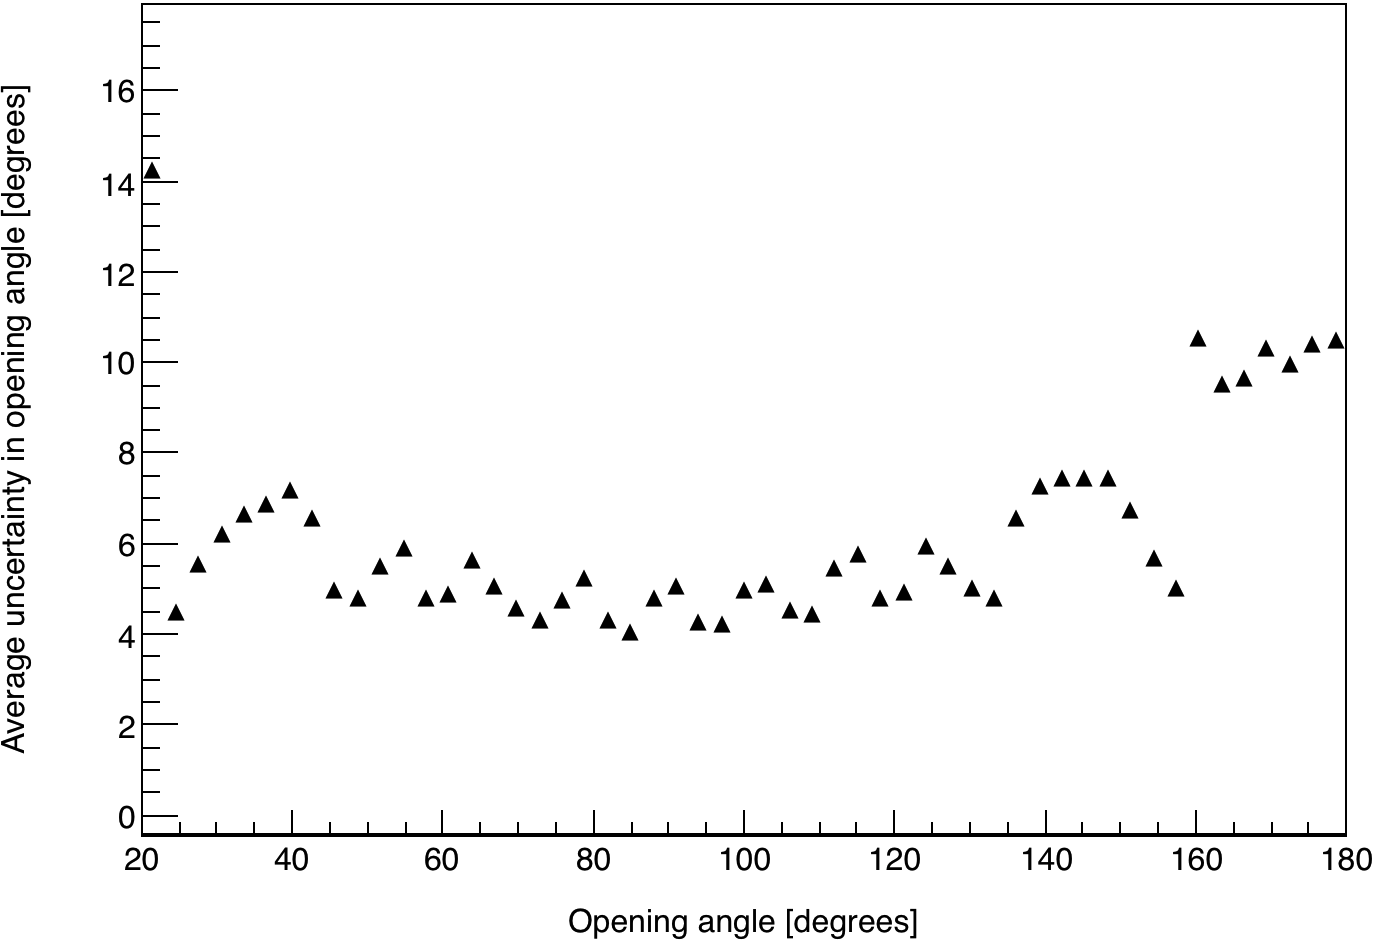
\includegraphics[width = 0.85\textwidth]{Content/Errors/OpeningAngleUncertainty.png}
    \caption{Uncertainties in opening angle determined from the propagation of position uncertainties through the opening angle calculation.
     %The uncertainty of a given opening angle measurement depends on which detectors are involved and the position of the particles on the detectors.
    % For this reason, the uncertainty of measurements falling within each angle bin is a distribution, so the average uncertainties are plotted here.
    The y-axis can be viewed as a measure of angular resolution in the sense that it represents the smallest angular difference that can be considered statistically significant.
    }
    \label{fig:OpeningAngleRes}
\end{figure}

\section{Counting error}
The uncertainty in the number of observed events is always assumed to be equal to $\sqrt{N}$, as per Poissonian  statistics, where N is the number of observed events.
This value is then propagated through the analysis procedure using the standard methods for the propagation of error.
The vertical error bars seen in all results are due solely to such counting error.

\FloatBarrier
\section{Detector Cross-talk}
\label{crosstalk}
\textit{Cross-talk} occurs when, after a particle is detected once, the same particle, by any means, causes a detection to be registered in a different detector.
For example, upon detection, a particle may undergo elastic scattering and then travel into a another detector where it is detected again, or it may produce secondary particles that are detected.
The two coincident detections of a cross-talk event are causally correlated, and thus they have the potential to contaminate the signal from correlated fission neutrons.
If both detections occur during the ToF range typical for fission neutrons, then the cross-talk event cannot be distinguished from the detection of two correlated neutrons.

Recent works that measured the two-neutron angular correlations in the spontaneous fission of $^{252}$Cf and $^{240}$Pu~\cite{Pozzi2016,Verbeke2018} addressed this effect by using an MCNP-PoLiMi simulation to estimate and then subtract cross-talk from their measurements.
In this work, the issue of cross-talk is approached differently by employing the use of detector shielding aimed at reducing cross-talk to a negligible rate.
By using shielding to reduce cross-talk, this measurement is less dependent on the details of the models used by MCNP-PoLiMi to simulate neutron transport and detection.
MCNP-PoLoMi simulations are used in this work only to verify that the effect of cross-talk is negligible.

The scintillators used here are much larger than those used in similar works, such as in refs~\cite{Pozzi2016,Verbeke2018}, allowing them to be placed much farther from the fission source without resulting in too low coincidence rates. 
An increase in the distance between the detectors and the fission source makes this measurement less sensitive to angular uncertainty, which depends directly on the uncertainty in the position of a detected particle due to, for example, the scattering of neutrons from detector shielding.
For this reason, larger amounts of shielding can be used without concern of introducing large errors.

The geometry of the neutron detection system makes it kinematically impossible for a neutron to scatter from a proton in one detector, which is the basis for scintillation, and then travel directly into another detector with enough kinetic energy to be detected a second time.
For this reason, upon being detected, a neutron must scatter from one or more intermediate nuclei, such as Pb or C, in order for it to reach another detector with enough energy to be detected again.
This fact follows from the conservation of energy and momentum.
Figure~\ref{fig:CrossTalkExample} illustrates a cross-talk event facilitated by the scattering of a neutron within a detector's shielding.
In order to increase the credibility of the claim that the design of the neutron detection system reduced cross-talk to negligible rates, a detailed MCNP-PoliMi~\cite{MCNP_POLIMI} simulation was performed in which a built-in $^{252}$Cf source is positioned at the center of a model of the neutron detection system.
\begin{figure}
    \centering
    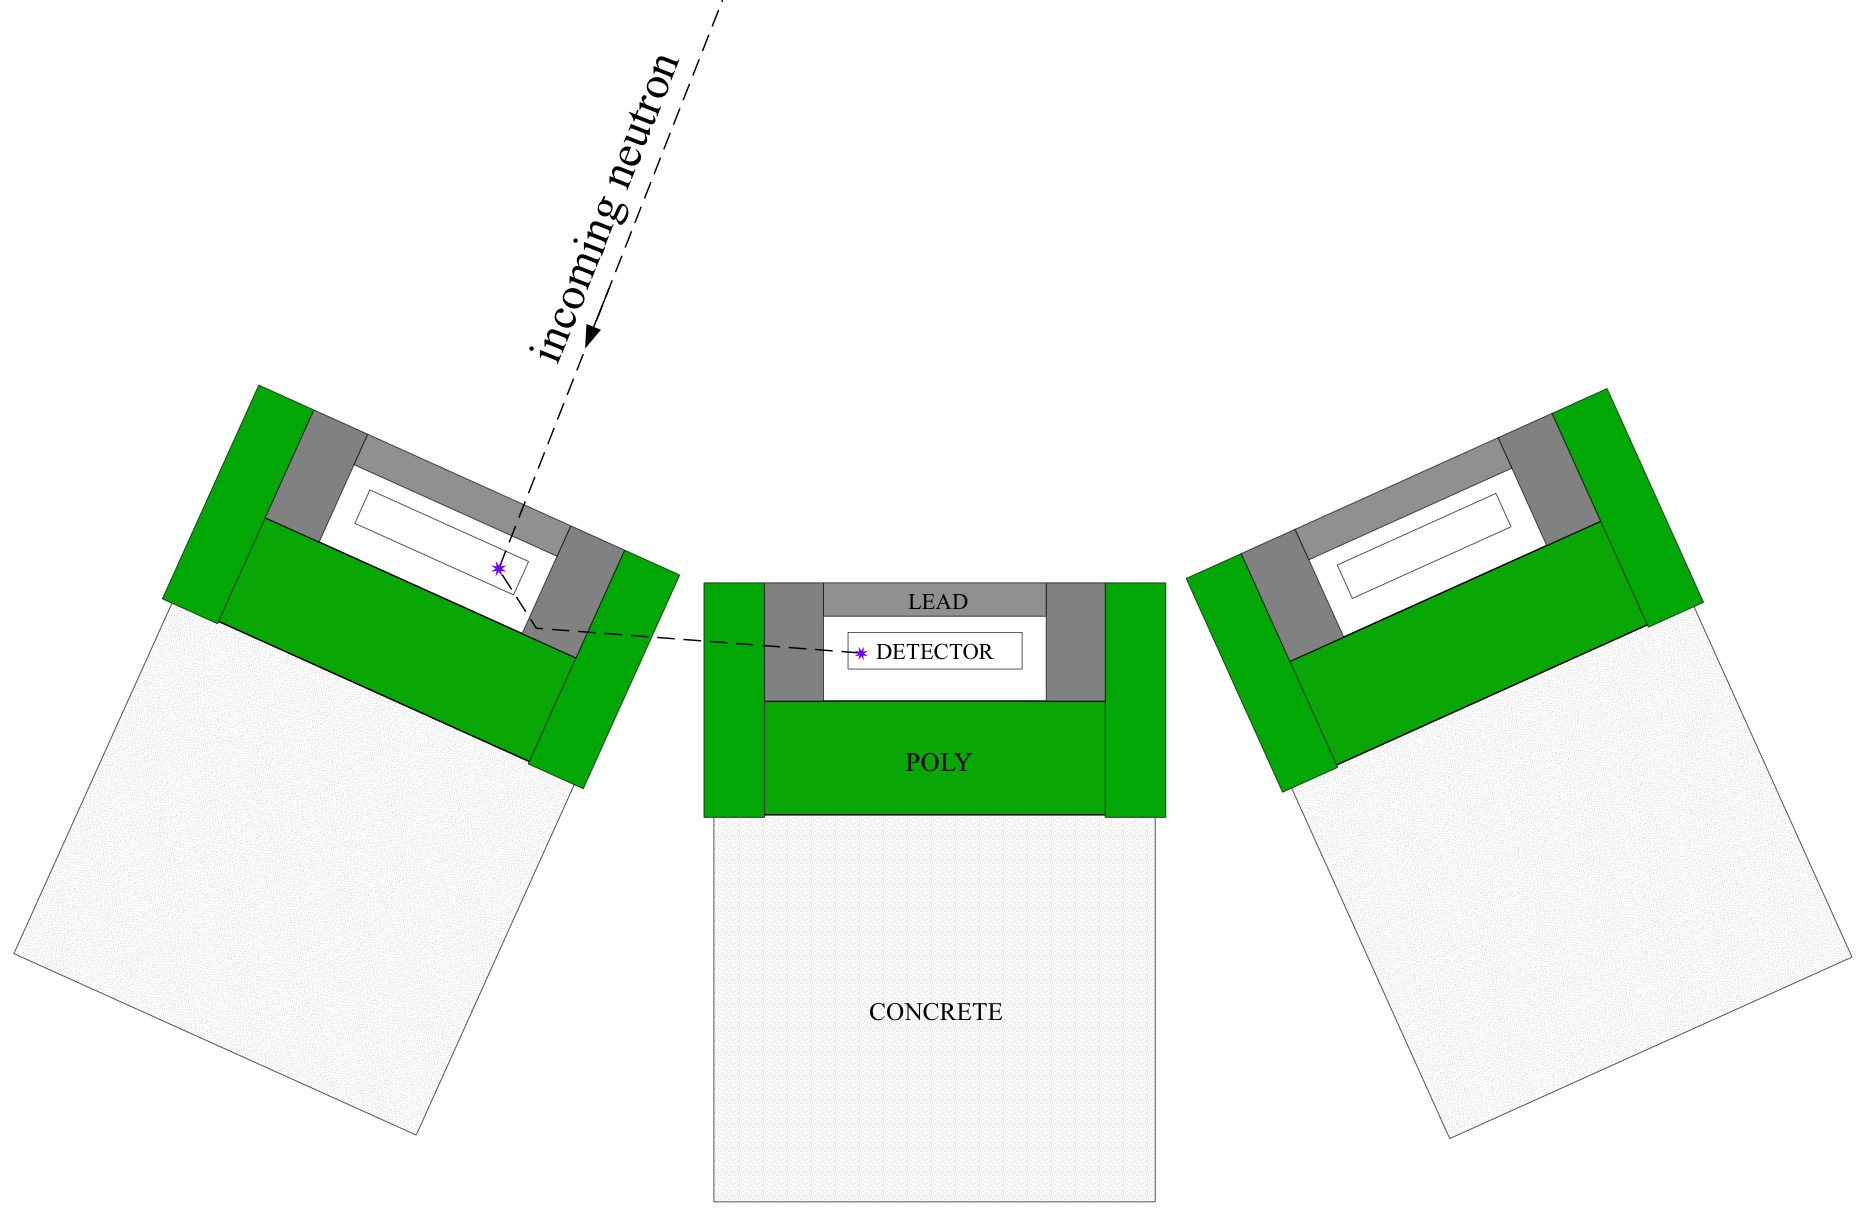
\includegraphics[width = 0.95\textwidth]{Content/Errors/CrossTalkExample.png}
    \caption{A hypothetical example of a neutron cross-talk event.
An incoming neutron is detected and then scatters from nearby lead shielding, changing its direction of travel such that it enters a second detector where it is detected a second time.
The scattering of a neutron from an intermediate nucleus, Pb in this example, is kinematically required in order for cross-talk to occur in this experiment.}
    \label{fig:CrossTalkExample}
\end{figure}

\subsection{Simulation of Detector Cross-talk}
The cross-talk simulation included all scintillators, shielding, detector supporting structures, and the concrete walls surrounding the experimental cell.
MCNP-PoliMi's built-in $^{252}$Cf spontaneous fission source was used, which emits neutrons with the correct correlations and multiplicities.
Detector response was modeled using a program included with the MCNP-PoliMi distribution called MPPost~\cite{MPPost}.
The model is based on the electron equivalent light output (MeVee) produced by particles as they undergo collisions with carbon and hydrogen within organic plastic scintillators.
A minimum deposited energy of 0.4 MeV (equivalent to 0.05 MeVee for neutrons) was assumed for detectable particles, which was chosen because the neutron detection system showed a sharp decline in detection rates for neutrons below 0.4 MeV.
For neutron collisions with hydrogen, the light output in MeVee, $L$, is calculated by the following empirically derived formula
\begin{displaymath}
L = 0.0364 E_n^2 +  0.125 E_n
\end{displaymath}
where $E_n$ is equal to the loss in the kinetic energy of the neutron due to the collision.
Neutron interactions with carbon are assumed to generate a small light output of
\begin{displaymath}
L = 0.02 E_n
\end{displaymath}
As seen in Fig.~\ref{fig:Cf252MCNPVsEXP}, this model of the detection process produces a ToF spectrum that is in good agreement with the measurement.
\begin{figure}
    \centering
    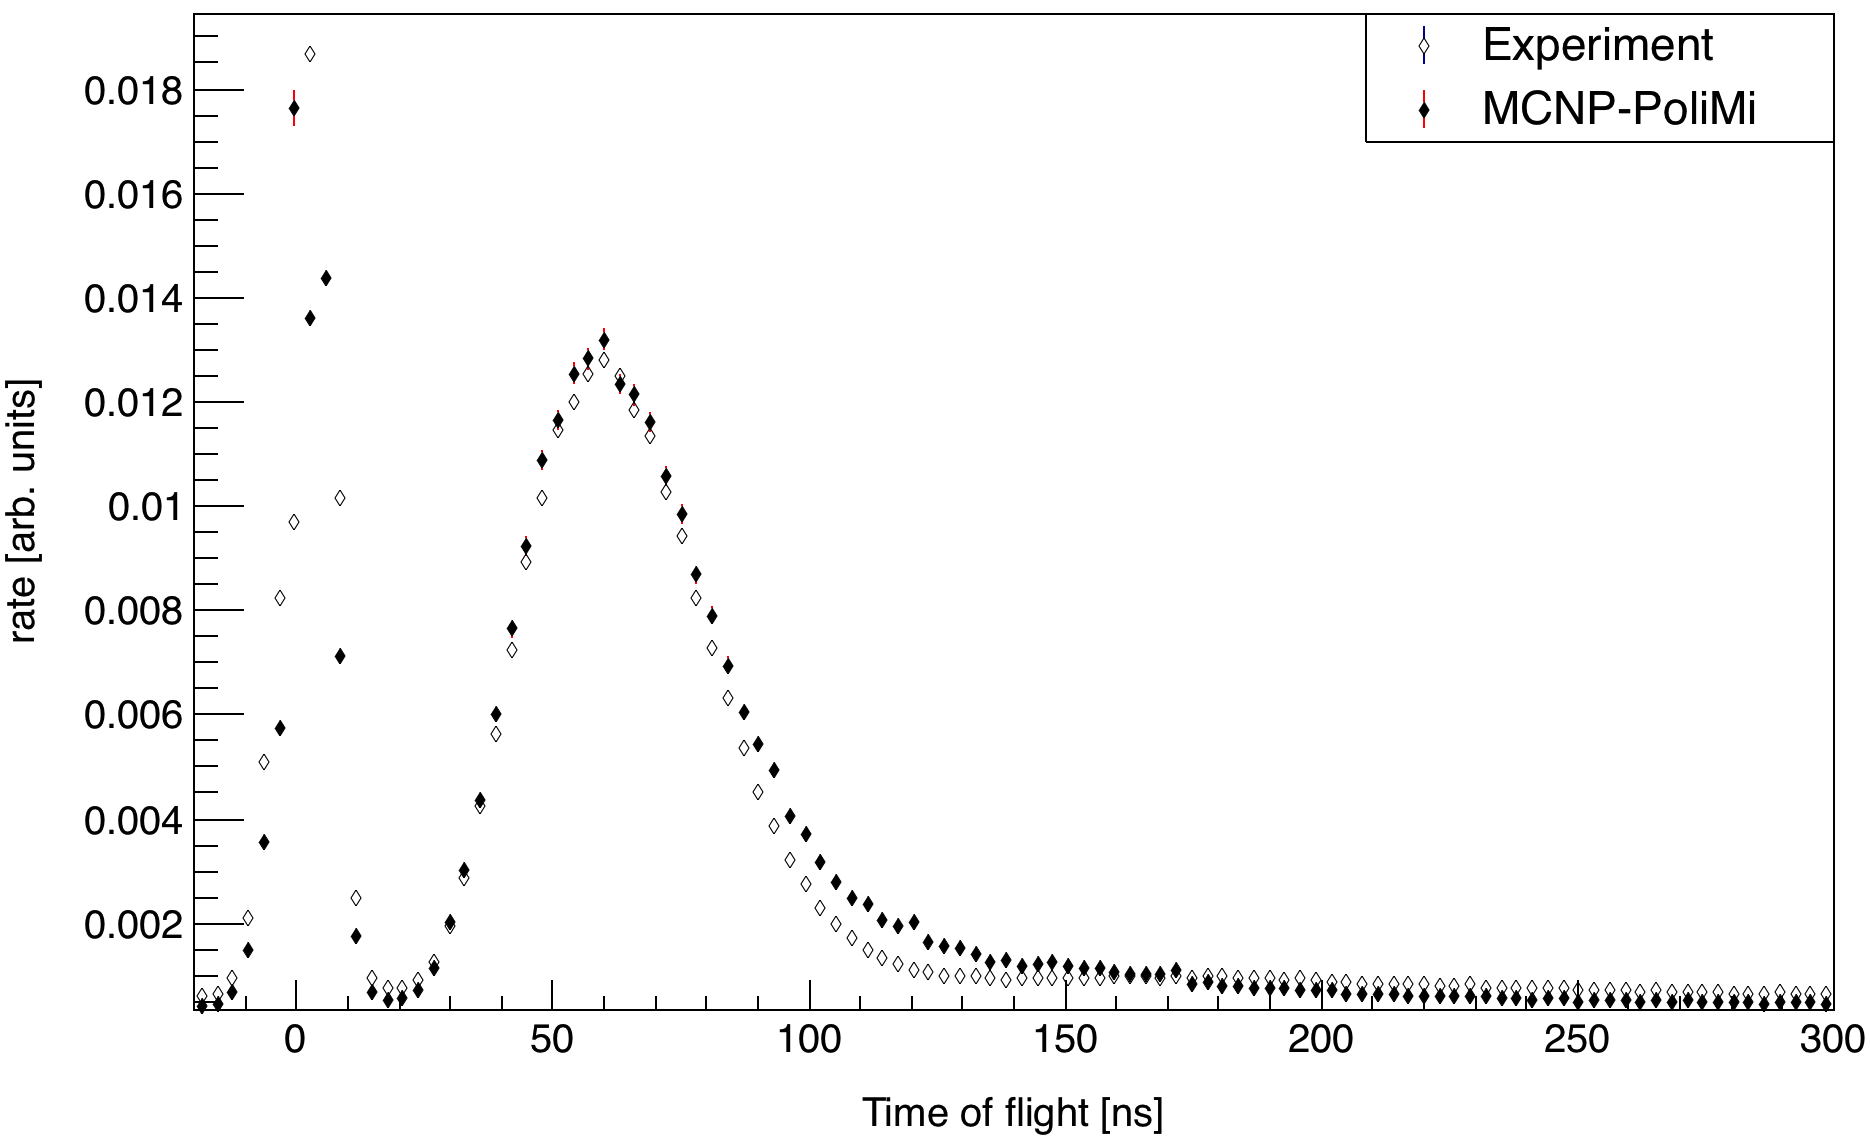
\includegraphics[width = 0.9\textwidth]{Content/Errors/Cf252MCNPVsEXP.png}
    \caption{Measured \emph{versus} simulated ToF spectrum from the SF of $^{252}$Cf, as reconstructed by the neutron detection system.
        The simulation used the detector response model outlined in ref~\cite{MPPost}}
    \label{fig:Cf252MCNPVsEXP}
\end{figure}

Figure~\ref{fig:CrosstalkVScoincidence} shows the distribution of cross-talk events and true two-neutron coincidences as a function of reconstructed opening angle.
It is worth noting that, according to this simulation, the effect of cross-talk is not only small, but is also distributed over a wide range of angles rather than being concentrated around $\theta_{nn}=0$.
Angles greater than 125 degrees are not shown in Fig.~\ref{fig:CrosstalkVScoincidence} because these cross-talk events can be readily identified in analysis due to the large amount of time required for a neutron to travel the these distances.
The simulation was initially performed with 5 cm of lead shielding placed behind the scintillators, and the number of cross-talk events accounted for 11\% of the total coincident neutron events.
This value fell to 3\% when polyethylene was used instead of lead, which is what motivated the placement of 10~cm of polyethylene behind the detectors instead of lead.
\begin{figure}
    \centering
    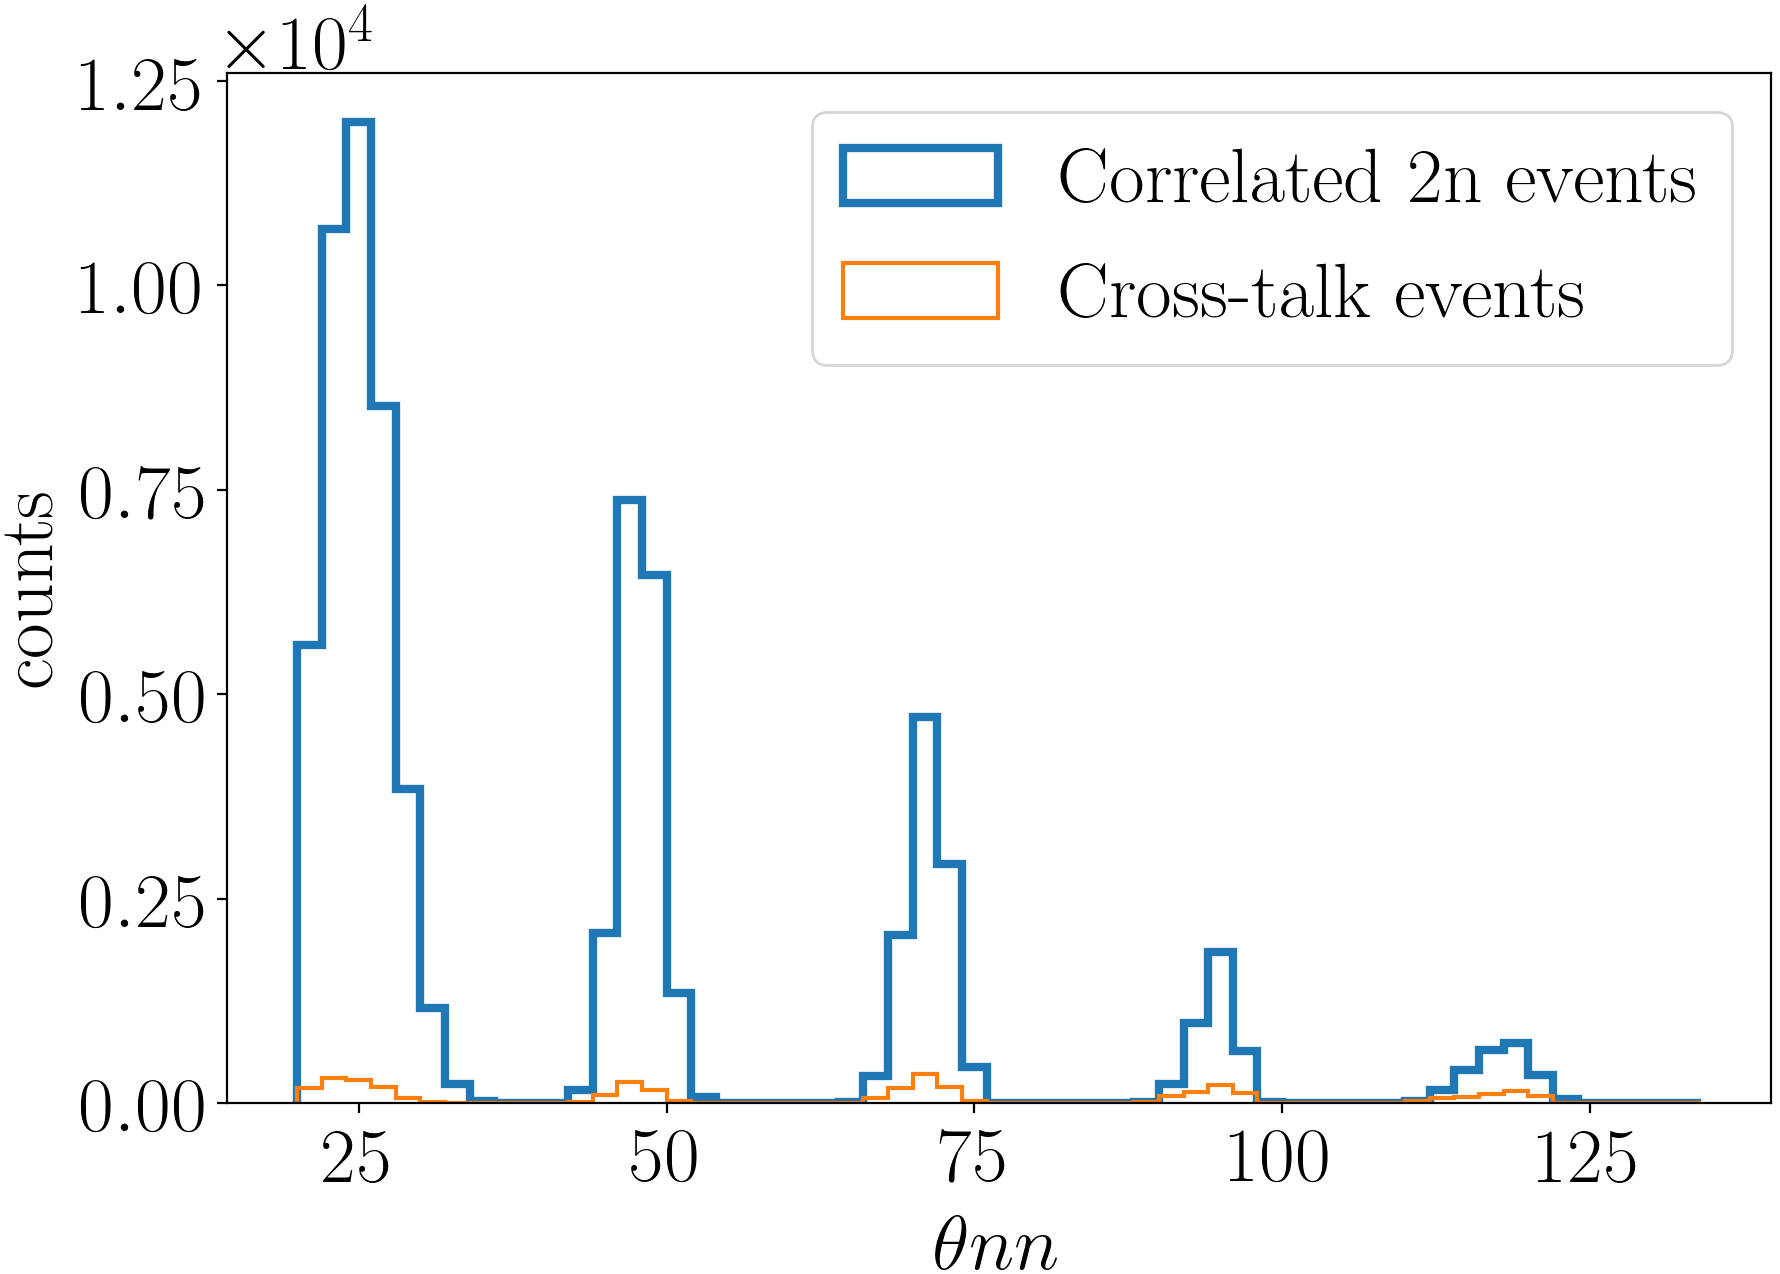
\includegraphics[width = 0.95\textwidth]{Content/Errors/CrosstalkVScoincidence.png}
    \caption{
    MCNP-PoLiMi simulation of the number of cross-talk events \emph{versus} correlated two-neutron events as a function of reconstructed opening angle.
    Cross-talk accounted for 3\% of total events.
    In this work, cross-talk does not occur primarily at small angles, but is instead spread out over a wide range of angles.
    }
    \label{fig:CrosstalkVScoincidence}
\end{figure}

\section{Neutron Scattering within Target}
\label{subsection:Elastic_scattering}
A potential source of error in opening angle measurements is the scattering of neutrons within the fission target.
This is a cause for concern because when neutrons scatter from heavy nucleons, such as $^{238}$U, they are likely to be deflected at large angles, resulting in two-neutron opening angles that do not reflect the true underlying fission kinematics.
The effect that the elastic scattering of neutrons within the target has on this work is assessed by MCNP simulations.
%Furthermore, because the target used in this work has the shape of a thin strip, it is more likely that neutrons emitted along the wide, 2~cm, axis of the strip undergo a scattering event than those emitted along the thinest, 0.05~cm, axis.
%As a result, detectors that are located collinear to the widest axis of the target will see relatively fewer neutrons due to increased scattering. 
%This bias is removed by slowly rotating the target about the vertical axis during data acquisition.
%Because the subject of this measurement is fundamentally a statistical process, useful interpretations of the data are average rates taken over many events.
%Thus, by rotating the target, cylindrical symmetry is preserved in the average to produce a result equivalent to that if a cylindrical target were used.

The target's dimensions are small enough that the rate of photon absorption, and thus photo-neutron production, is virtually uniform throughout the entire target volume.
Accordingly, an MCNP-PoLiMi simulation was used to generate $^{252}$Cf spontaneous fission events uniformly throughout the target.
The SF of $^{252}$Cf is used instead of the photofission of $^{238}$U because of the current lack of photofission models, however, the underlying fission kinematics are, broadly speaking, the same for the SF of $^{252}$Cf and the photofission of $^{238}$U, thus, the two process have similar neutron-neutron correlations.
The probability that at least one neutron out of a pair of two scatters before exiting the target was calculated from the simulation, indicating that 6\% of measured two-neutron opening angles were perturbed due to scattering.

The rate of elastic scattering is affected by the size and shape of the target.
A thin strip is the ideal target shape regarding the rate of neutron elastic scattering per unit of total target volume.
See Fig~\ref{fig:ElasticScatteringPlot} for the simulated elastic scattering rates for both thin strip and cylindrical shaped targets.
The simulation indicated that the rate of elastic scattering in cylindrical targets is about a factor of two times greater than in thin strip targets with the same volume and a width-to-thickness ratio of 40.

\begin{figure}
    \centering
    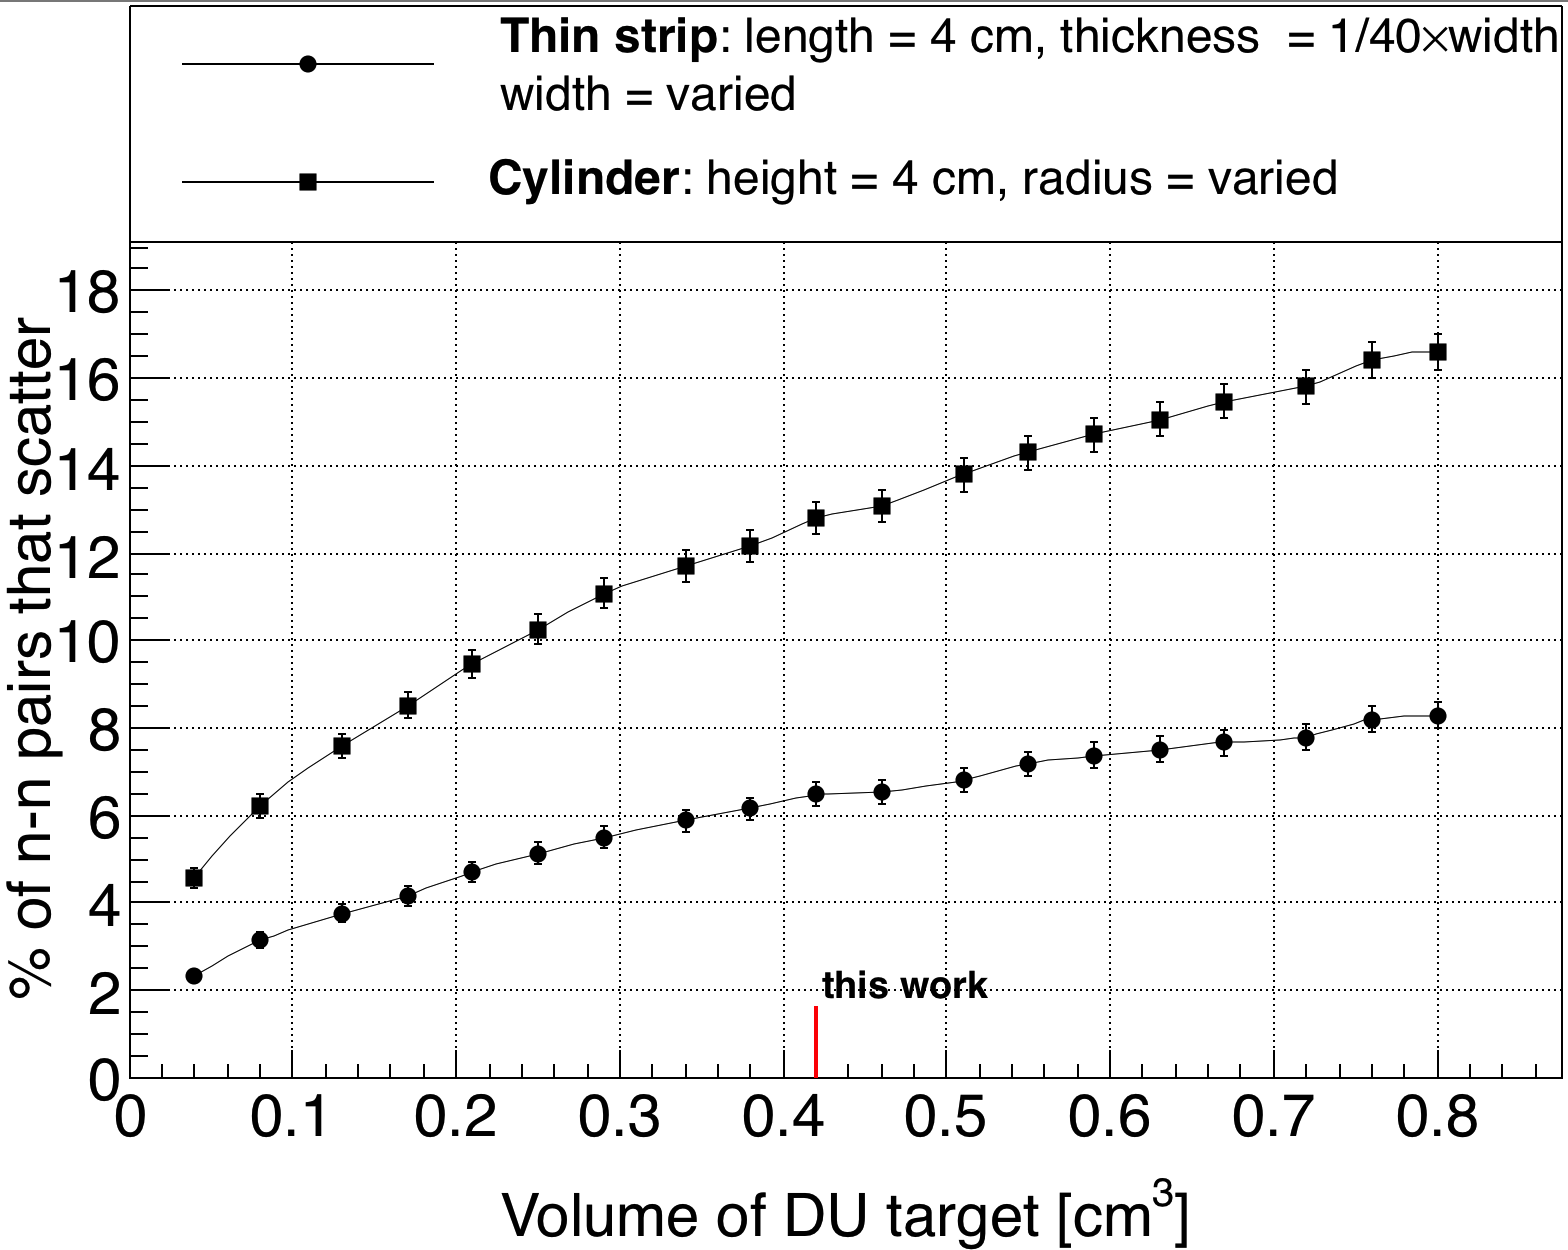
\includegraphics[width = 0.95\textwidth]{Content/Errors/ElasticScatteringPlot.png}
    \caption{
     Result of an MCNP simulation in which neutron-neutron pairs, with energies sampled from a typical watt fission spectrum, were generated uniformly throughout the volume of DU targets.
        The y-axis is the rate of opening angle contamination due to the scattering of, within the DU target in which they were produced, either one or both of a pair of neutrons.
    The lack of symmetry of a thin strip target can be removed by slowly rotating the target around the vertical axis during data acquisition, making it the optimal target geometry for the minimization of the rate of neutron scattering.
    The target used in this work had a length of 4~cm, a width of 2~cm, and a thickness of 0.05~cm.
    }
    \label{fig:ElasticScatteringPlot}
\end{figure}

Section~\ref{sec:anomaly} discusses the observation of an unexpected drop in correlation around 180$^{\circ}$ in our photofission of $^{238}$U measurement, as seen in Figs.~\ref{fig:DU(0)}-\ref{fig:DU(1)}.
This motivated a second simulation regarding elastic scattering which examined whether this decrease in the correlation around 180$^{\circ}$ opening angles reflects the underlying physics of the fission process.
In particular, note that throughout these measurements, the target was continuously rotated once per 8 seconds.
This means that for the determination of the uncorrelated opening angle distribution, the trajectories of the two neutrons were taken from two different pulses in which the target was at a different orientation for each of them.
Additionally, each of the neutrons likely originated from different regions of the target volume.
On the other hand, for the same-pulse, correlated neutron measurement, the target was in the same orientation and the two neutrons were generated at the same position in the target.
For these reasons, the rates of neutron scattering within the target are not necessarily equal for the same-pulse and different-pulse cases.
As such, we investigated whether these differences could cause this apparent decrease in the opening angle distribution.

Using the correlated $^{252}$Cf SF source built-in to MCNP-PoLiMi, the opening angle distribution of neutrons at the moment of emission were compared to that the neutrons after they have escaped the target.
The location of fission events were sampled uniformly throughout the targets volume.
The analysis employs the same technique outlined in section~\ref{subsec:SPDPCancelation}, in which a correlated neutron distribution is divided by an uncorrelated neutron distribution.
The angular correlation is calculated by pairing neutrons emitted during the same fission, and the uncorrected distribution by the pairing of neutrons emitted during different fissions.
In order to account for the effect of a rotating target on the trajectories of neutrons from different-pulses, the coordinate system was rotated about the vertical axis accordingly for different fission events.

Aside from the size, shape, and continuous rotation of the target, the rate of neutron scattering within the target of detected neutrons is also affected by the fact that the detection system does not have 4$\pi$ coverage.
The target is itself asymmetrical, and thus not all exit trajectories for a photo-neutrons are created equal regarding the scattering probability.
The detection system's limited geometrical coverage has the potential to favor some neutron trajectories over others, possibly causing a relatively higher rate of the measurement of scattered n-n pairs for particular opening angles.
The potential for this to affect the measurement is captured in the simulation by only counting neutrons which enter a physical volume at which a detector was located during the experiment.
This distribution is labeled \emph{reconstructed} in Fig.~\ref{fig:ElasticScatteringEffect}, and includes the effects of neutron elastic scattering within the target together with the geometric coverage of the neutron detection system.
Plotted alongside the reconstructed distribution is the opening angle distribution of the neutrons at the moment immediately after emission, labeled \emph{true}.
A neutron energy cut of 0.4 MeV is applied to all neutrons in both cases in order to be more reflective of the measurement.
%Fig~\ref{fig:ElasticScatteringEffect} compares the two-neutron opening angle distribution at the moment immediately after emission (denoted by \emph{true} in figure) to that of neutrons once they have escaped the target (denoted by \emph{reconstructed} in figure).
From this simulation it was concluded that the rotating 0.05$\times$2$\times$4~cm$^3$ U-238 target does not, due to neutron scattering, result in a significant departure from the true opening angle distribution.
\begin{figure}
    \centering
    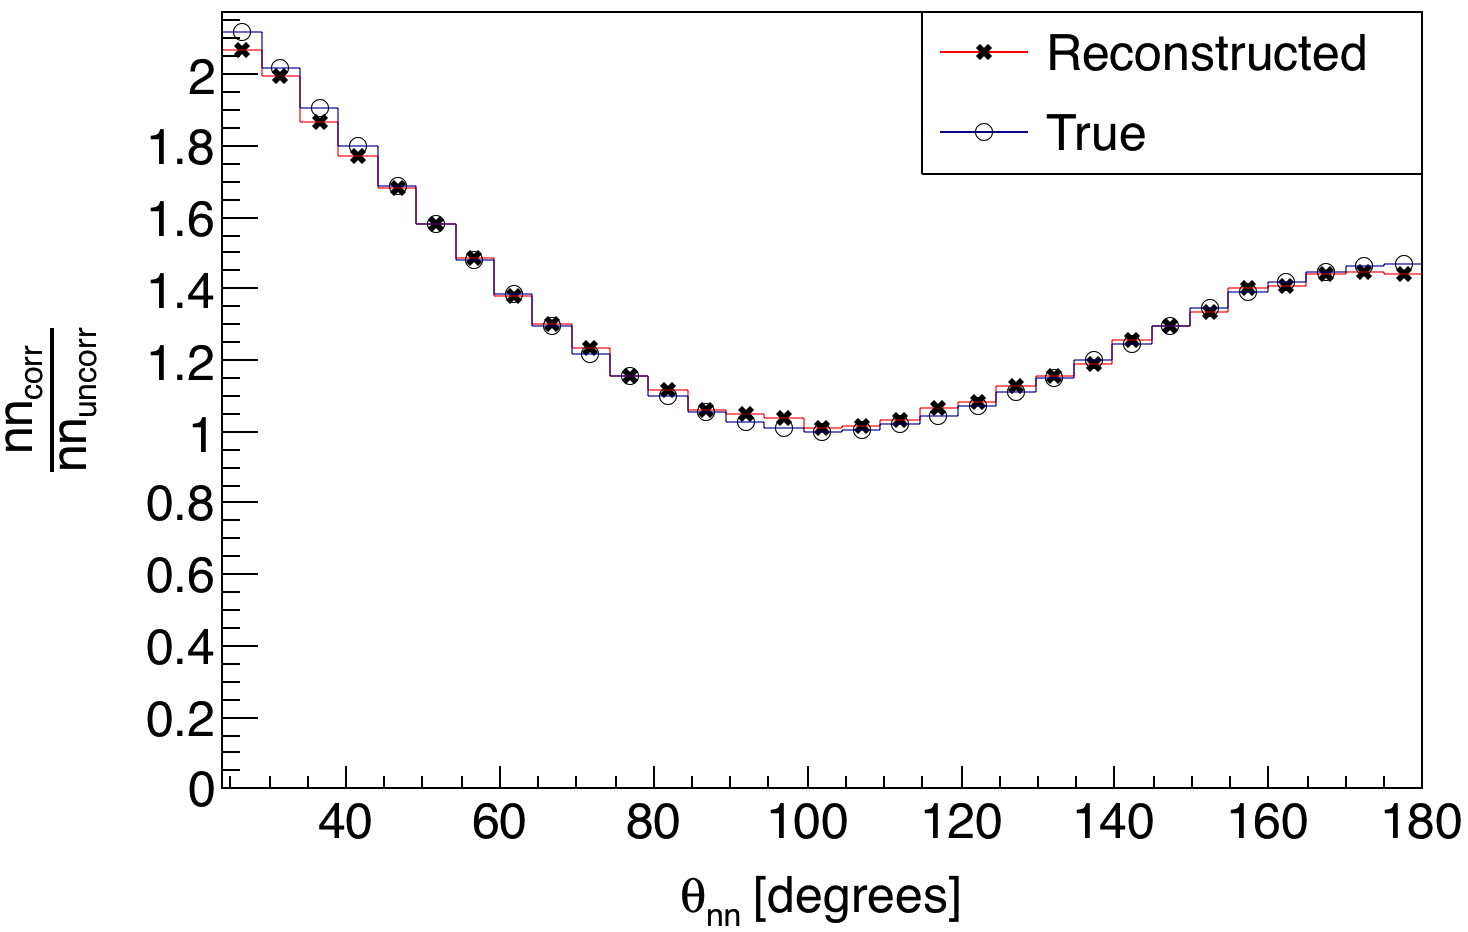
\includegraphics[width = 0.95\textwidth]{Content/Errors/EffectOfElasticScattering.png}
    \caption{
    MCNP-PoLiMi simulation of correlated $^{252}$Cf neutrons sampled uniformly throughout a 0.05$\times$2$\times$4~cm$^3$ U-238 target.
    A neutron cut of 0.4 MeV is applied to all neutrons as to more closely reflect the experiment.
    The slight difference between the curves is due solely to the elastic scattering of neutrons within the target, since detector physics was not simulated.
    In the reconstructed $\theta_{nn}$ distribution ({\tiny \ding{54}}), only neutrons which enter a physical volume at which a detector was located during the experiment are counted.
   The true $\theta_{nn}$ distribution at the moment of emission is also plotted ($\mathlarger{\mathlarger{\mathlarger{\circ}}}$).
    }
    \label{fig:ElasticScatteringEffect}
\end{figure}